\documentclass[tikz]{tmr}
\usepackage{mathtools}
\usepackage{amsthm}
\usepackage{tikz}
\usepackage{lscape}
\usepgflibrary{shapes.multipart}
\usepackage{listings} % package `semantic` does not work with class `tmr`
\usepackage{stmaryrd} % for \{ll,rr}bracket	

\lstdefinestyle{demo}{numbers=none,frame=,moredelim=[is][\color{brown}]{\{\{}{\}\}}}
%\lstset{style=literateHaskell,numbers=left,numberstyle=\tiny,frame=lines}
\lstset{
language=haskell,
numbers=left,
numberstyle=\tiny,
frame=lines,
tabsize=4,
basicstyle=\ttfamily\small,
literate=*{|}{$\vert$}{1}
}

\title{The SC~Mini Supercompiler}
\subtitle{Appendix to the article ``Supercompilation: Ideas and Methods''}
\author{Ilya Klyuchnikov\email{ilya.klyuchnikov@gmail.com}}
\author{Dimitur Krustev\email{dkrustev@gmail.com}}

%\maketitle

\begin{document}

%\title{Суперкомпилятор SC Mini}
%\subtitle{Приложение к статье <<Суперкомпиляция: идеи и методы>>}
%\author{Илья Ключников}
%
%\maketitle

\begin{introduction}
%\noindent This appendix lists the full sources of SC Mini (except for module and import declarations),
%with explanations of the technical details of the implementation.
%
%\null

\noindent The internals of the supercompiler SC Mini are explained step by step in this appendix.
\end{introduction}

%\tableofcontents
\section*{Introduction}

The SC Mini sources can -- somewhat subjectively -- be divided into the following parts:
\begin{enumerate}
  \item Data type definitions with some basic operations: SLL abstract syntax;
  basic operations on SLL expressions; definition of a SLL ``task''
  and ``graph of configurations''.
  	\begin{itemize}
  	\item \texttt{Data.hs}
  	\end{itemize}
  \item Auxiliary functions for working with the main data structures: parser, substitutions, expression comparison, etc.
  	\begin{itemize}
  	\item \texttt{DataUtil.hs}
  	\end{itemize}
  \item Main part -- interpreter, driving, folding, transformers \texttt{transform},
  \texttt{deforest} and \texttt{supercompile}, residual task generator.
  	\begin{itemize}
  	 \item \texttt{Interpreter.hs}
  	 \item \texttt{Driving.hs}
  	 \item \texttt{TreeInterpreter.hs}
  	 \item \texttt{Folding.hs}
  	 \item \texttt{Generator.hs}
  	 \item \texttt{Prototype.hs}
  	 \item \texttt{Deforester.hs}
  	 \item \texttt{Supercompiler.hs}
  	\end{itemize}
  \item A set of examples together with their results.
  	\begin{itemize}
  	\item \texttt{Demonstration.hs}
  	\end{itemize}
\end{enumerate}

The full SC Mini sources are listed, only the parsers/pretty-printers are omitted.
New definitions are illustrated with actual output from running them.
All interesting examples are collected in the module \texttt{Demonstration.hs}. 
The reader can also download and directly play with the actual sources.
%Читатель может самостоятельно запустить пример и
%убедиться в его работоспособности -- везде указывается функция (\texttt{demo01}, \texttt{demo02},
%\ldots), вызвав которую из интерпретатора ghci, читатель получит тот же результат, что здесь.

For convenience, we recall here the definition of SLL operational semantics.

\begin{figure}[h!]
\begin{tabular}{l r l}
%$obs$ & ::= & $C(e_1, \ldots, e_n)$ $\mid$ $v$ \\
$con$ & ::= & $\langle\rangle$
			$\mid$ $g(con, \ldots)$\\
$red$ & ::= & $f(e_1, \ldots, e_n)$
			$\mid$ $g(C(e_1, \ldots, e_n), \ldots)$
			$\mid$ $g(v, \ldots)$
\end{tabular}
\caption{SLL: expression decomposition}
\label{fig:sll_decomposition}
\end{figure}

\begin{figure}[h!]
\begin{tabular}{l l l}
$\mathcal{I} \llbracket e \rrbracket$ &
$\Rightarrow$ &
$e$ \\ & & if $e$ is a value\\

$\mathcal{I} \llbracket C(e_1, \ldots, e_n) \rrbracket$ &
$\Rightarrow$ &
$C(\mathcal{I} \llbracket e_1 \rrbracket, \ldots, \mathcal{I} \llbracket e_n \rrbracket)$ \\

$\mathcal{I} \llbracket con \langle f(e_1, \ldots, e_n) \rangle \rrbracket$ &
$\Rightarrow$ &
$\mathcal{I} \llbracket con \langle e \{v_1 := e_1, \ldots, v_n := e_n\} \rangle \rrbracket$ \\
& & when $f(x_1, \ldots, x_n) \stackrel{\textrm{\tiny p}}{=} e$\\

$\mathcal{I} \llbracket con \langle g(C(e_1, \ldots, e_m), e_{m+1},\ldots, e_n)\rangle \rrbracket$ &
$\Rightarrow$ &
$\mathcal{I} \llbracket con \langle e \{v_1 := e_1, \ldots, v_n := e_n\} \rangle \rrbracket$ \\
& & when $g(C(v_1, \ldots, v_m), v_{m+1},\ldots, v_n) \stackrel{\textrm{\tiny p}}{=} e$ 
\end{tabular}
\caption{Reduction step rules}
\label{fig:sll_semantics}
\end{figure}
\section{\texttt{Data.hs}}

First a definition of SLL abstract syntax. To make generalization easier, it
already includes \texttt{let}-expressions.
\begin{lstlisting}[name=data]
type Name = String
data Expr = Var Name | Ctr Name [Expr] | FCall Name [Expr] 
	| GCall Name [Expr] | Let (Name, Expr) Expr 
	deriving (Eq)
data Pat = Pat Name [Name] deriving (Eq)
data GDef = GDef Name Pat [Name] Expr deriving (Eq)
data FDef = FDef Name [Name] Expr deriving (Eq)
data Program = Program [FDef] [GDef] deriving (Eq)
\end{lstlisting}

Type synonyms for operations on expressions: renaming, substitution, fresh-name supply.
\begin{lstlisting}[name=data]
type Renaming = [(Name, Name)]
type Subst = [(Name, Expr)]
type NameSupply = [Name]
\end{lstlisting}

Technically we work with SLL-expressions almost everywhere. 
But to distinguish in which sense we use them --
expression, configuration, value --
we introduce some more type synonyms:
\begin{lstlisting}[name=data]
type Conf = Expr
type Value = Expr
type Task = (Conf, Program)
type Env = [(Name, Value)]
\end{lstlisting}

Probably the most interesting data types:
\begin{lstlisting}[name=data]
data Contract = Contract Name Pat
data Step a = Transient a | Variants [(Contract, a)] | Stop 
	| Decompose [a] | Fold a Renaming
data Graph a = Node a (Step (Graph a))
type Tree a = Graph a
type Node a = Tree a

type Machine a = NameSupply -> a -> Step a
\end{lstlisting}

In the following we shall consider the processed program as a kind of machine.
\texttt{Machine~a} operates with some generalized states of type \texttt{a}.
We assume further, that states can contain named subparts (using identifiers), and that
the machine may need to produce some new named subparts.
If the machine is given some infinite list of names and some current state,
then it computes in one step a next generalized state.
The data type \texttt{Step~a} describes the kinds of steps we use
-- transient, final, decomposition, etc. 
The most interesting kind of step -- \texttt{Variants~[(c1,~a1),~(c2,~a2),\ldots]}
~-- describes case analysis. 
Its meaning is: if the condition \texttt{c1} holds, then the next state will be \texttt{a1},
if \texttt{c2} holds -- \texttt{a2}, etc.
We consider only simple conditions of type \texttt{Contract} --
namely that some variable matches a certain pattern.
\texttt{Graph~a}~-- is the graph of state transitions.

We shall use further only configurations as states, but the type of state
is deliberately abstracted here for full generality.

\section{\texttt{DataUtil.hs}}

The module \texttt{DataUtil} defines some (mostly boring) auxiliary functions. 
Its text is included for completeness anyway.

Working with abstract syntax:
\begin{lstlisting}[name=datautil]
isValue :: Expr -> Bool
isValue (Ctr _ args) = and $ map isValue args
isValue _ = False

isCall :: Expr -> Bool
isCall (FCall _ _) = True
isCall (GCall _ _) = True
isCall _ = False

isVar :: Expr -> Bool
isVar (Var _) = True
isVar _ = False

fDef :: Program -> Name -> FDef
fDef (Program fs _) fname = 
	head [f | f@(FDef x _ _) <- fs, x == fname]

gDefs :: Program -> Name -> [GDef]
gDefs (Program _ gs) gname = 
	[g | g@(GDef x _ _ _) <- gs, x == gname]

gDef :: Program -> Name -> Name -> GDef
gDef p gname cname = 
	head [g | g@(GDef _ (Pat c _) _ _) <- 
		gDefs p gname, c == cname]
\end{lstlisting}

Applying substitutions:
\begin{lstlisting}[name=datautil]
(//) :: Expr -> Subst -> Expr
(Var x) // sub = maybe (Var x) id (lookup x sub)
(Ctr name args) // sub = Ctr name (map (// sub) args)
(FCall name args) // sub = FCall name (map (// sub) args)
(GCall name args) // sub = GCall name (map (// sub) args)
(Let (x, e1) e2) // sub  = Let (x, (e1 // sub)) (e2 // sub)
\end{lstlisting}

Working with names.
\texttt{nameSupply} produces an infinite list of names. 
\texttt{unused} removes from the list of names those used inside a condition.
\texttt{vnames'} -- all the names inside an expression, \texttt{vnames} -- the same without repetitions. 
\texttt{isRepeated} checks if a name occurs more than once in an expression.
\begin{lstlisting}[name=datautil]
nameSupply :: NameSupply
nameSupply = ["v" ++ (show i) | i <- [1 ..] ]

unused :: Contract -> NameSupply -> NameSupply
unused (Contract _ (Pat _ vs)) = (\\ vs)

vnames :: Expr -> [Name]
vnames = nub . vnames'

vnames' :: Expr -> [Name]
vnames' (Var v) = [v]
vnames' (Ctr _ args)   = concat $ map vnames' args
vnames' (FCall _ args) = concat $ map vnames' args
vnames' (GCall _ args) = concat $ map vnames' args
vnames' (Let (_, e1) e2) = vnames' e1 ++ vnames' e2

isRepeated :: Name -> Expr -> Bool
isRepeated vn e = (length $ filter (== vn) (vnames' e)) > 1
\end{lstlisting}

%\newpage
\texttt{renaming e1 e2} finds a renaming (if possible) from an expression \texttt{e1} 
into an expression \texttt{e2}
(probably a more elegant definition is possible):
\begin{lstlisting}[name=datautil]
renaming :: Expr -> Expr -> Maybe Renaming
renaming e1 e2 = 
	f $ partition isNothing $ renaming' (e1, e2) where
	f (x:_, _) = Nothing
	f (_, ps) = g gs1 gs2
		where
			gs1 = groupBy (\(a, b) (c, d) -> a == c) 
				$ sortBy h $ nub $ catMaybes ps
			gs2 = groupBy (\(a, b) (c, d) -> b == d) 
				$ sortBy h $ nub $ catMaybes ps
			h (a, b) (c, d) = compare a c
	g xs ys = 
		if all ((== 1) . length) xs 
			&& all ((== 1) . length) ys
		then Just (concat xs) else Nothing

renaming' :: (Expr, Expr) -> [Maybe (Name, Name)]
renaming' ((Var x), (Var y)) =
	[Just (x, y)]
renaming' ((Ctr n1 args1), (Ctr n2 args2)) | n1 == n2 =
	concat $ map renaming' $ zip args1 args2
renaming' ((FCall n1 args1), (FCall n2 args2)) | n1 == n2 =
	concat $ map renaming' $ zip args1 args2
renaming' ((GCall n1 args1), (GCall n2 args2)) | n1 == n2 =
	concat $ map renaming' $ zip args1 args2
renaming' (Let (v, e1) e2, Let (v', e1') e2') =
	renaming' (e1, e1') ++ 
		renaming' (e2, e2' // [(v, Var v')])
renaming' _  = [Nothing]
\end{lstlisting}
Expression size (used inside the whistle):
\begin{lstlisting}[name=datautil]
size :: Expr -> Integer
size (Var _)          = 1
size (Ctr _ args)     = 1 + sum (map size args)
size (FCall _ args)   = 1 + sum (map size args)
size (GCall _ args)   = 1 + sum (map size args)
size (Let (_, e1) e2) = 1 + (size e1) + (size e2)
\end{lstlisting}
Other utility functions:
\begin{lstlisting}[name=datautil]
nodeLabel :: Node a -> a
nodeLabel (Node l _) = l

step :: Node a -> Step (Graph a)
step (Node _ s) = s
\end{lstlisting}
\section{\texttt{Interpreter.hs}}
The module \texttt{Interpreter} defines an evaluator for SLL expressions.

The interpreter \texttt{int} works in ``small-step'' fashion, or in other words,
reduction steps are repeated until the expression becomes a value.
(\texttt{intStep}) implements a single reduction step; note that it is not recursive.
\begin{lstlisting}[name=interpreter]
int :: Program -> Expr -> Expr
int p e = until isValue (intStep p) e

intStep :: Program -> Expr -> Expr
intStep p (Ctr name args) =
	Ctr name (values ++ (intStep p x : xs)) where
		(values, x : xs) = span isValue args

intStep p (FCall name args) =
	body // zip vs args where
		(FDef _ vs body) = fDef p name

intStep p (GCall gname (Ctr cname cargs : args)) =
	body // zip (cvs ++ vs) (cargs ++ args) where
		(GDef _ (Pat _ cvs) vs body) = gDef p gname cname

intStep p (GCall gname (e:es)) =
	(GCall gname (intStep p e : es))

intStep p (Let (x, e1) e2) =
	e2 // [(x, e1)]
\end{lstlisting}

The interpreter \texttt{eval}, on the other hand, is a ``big-step'' evaluator,
and hence -- recursive.
\begin{lstlisting}[name=interpreter]
eval :: Program -> Expr -> Expr
eval p (Ctr name args) =
	Ctr name [eval p arg | arg <- args]

eval p (FCall name args) =
	eval p (body // zip vs args) where
		(FDef _ vs body) = fDef p name

eval p (GCall gname (Ctr cname cargs : args)) =
	eval p (body // zip (cvs ++ vs) (cargs ++ args)) where
		(GDef _ (Pat _ cvs) vs body) = gDef p gname cname

eval p (GCall gname (arg:args)) =
	eval p (GCall gname (eval p arg:args))

eval p (Let (x, e1) e2) =
	eval p (e2 // [(x, e1)])
\end{lstlisting}

For the small-step interpreter it is easy to count the number of performed reduction steps
-- it is enough to introduce a counter in the outer loop.
\texttt{intC} returns a pair \texttt{(value,~n)}, where \texttt{value} is a (surprise!) value,
and \texttt{n} -- the number of reduction steps performed.
This number is used to measure optimization ``speed-up''.
\begin{lstlisting}[name=interpreter]
sll_run :: Task -> Env -> Value
sll_run (e, program) env = int program (e // env)

sll_trace :: Task -> Subst -> (Value, Integer)
sll_trace (e, prog) s = intC prog (e // s)

intC :: Program -> Expr -> (Expr, Integer)
intC p e = until t f (e, 0) where
	t (e, n) = isValue e
	f (e, n) = (intStep p e, n + 1)
\end{lstlisting}

% \begin{lstlisting}[escapechar=!,style=demo]
% prog1 = !\fbox{\parbox{18em}{
% add(Z(), y) = y;\\
% add(S(x), y) = S(add(x), y);\\
% mult(Z(), y) = Z();\\
% mult(S(x), y) = add(y, mult(x, y));\\
% sqr(x) = mult(x, x);\\
% gEven(Z()) = True();\\
% gEven(S(x)) = gOdd(x);\\
% gOdd(Z()) = False();\\
% gOdd(S(x)) = gEven(x);}}!
% \end{lstlisting}

%\newpage

From now on we start illustrating the definitions discussed with example runs.
Each such example is actually a separate function definition in the module \texttt{Demonstration}.
It is useful to distinguish SLL code from Haskell code.
To this end, SLL code is presented in color.
(Actually in \texttt{Demonstration.hs} SLL code appears as strings, which are parsed:
\texttt{{\color{brown}{even(x)}}} $\Rightarrow$ \texttt{read "even(x)"} )

The first example evaluates an expression, and also returns the number of reduction steps:
\begin{lstlisting}[style=demo]
-- demo01
ghci> intC prog1 {{even(sqr(S(S(Z()))))}}
(True(), 15)
\end{lstlisting}

The next examples show that the small-step and the big-step interpreter give the same result:
\begin{lstlisting}[style=demo]
-- demo02
ghci> int  prog1 {{even(sqr(S(S(Z()))))}}
True()

-- demo03
ghci> eval prog1 {{even(sqr(S(S(Z()))))}}
True()

-- demo04
ghci> int  prog1 {{sqr(S(S(Z())))}}
S(S(S(S(Z()))))

-- demo05
ghci> eval prog1 {{sqr(S(S(Z())))}}
S(S(S(S(Z()))))
\end{lstlisting}

A difference between the 2 interpreters appears, if we try to evaluate an expression
with free variables (a configuration).
\texttt{int} only signals an exception. 
\texttt{eval}, on the other hand, returns some information before signaling failure:
\begin{lstlisting}[style=demo]
-- demo06
ghci> int  prog1 {{sqr(S(S(x)))}}
Exception: Interpreter.hs: Non-exhaustive patterns in 
function intStep

-- demo07
ghci> eval  prog1 {{sqr(S(S(x)))}}
S(S( Exception: Interpreter.hs: Non-exhaustive patterns 
in function eval
\end{lstlisting}

The difference is even more dramatic, if we try to evaluate an expression, which has an infinite value.
\texttt{int} directly loops, while \texttt{eval} starts to produce the outermost constructors
of the result.)
\begin{lstlisting}[style=demo]
ghci> prog3 = {{inf() = S(inf());}}
inf() = S(inf());

-- demo08
ghci> int prog3 {{inf()}}
^CInterrupted.

-- demo09
ghci> eval prog3 {{inf()}}
S(S(S(S(S(S(S(S(S(S(S(S(S(S(S(S(S(S(S(S(S(S(S(S(S(S(S(S(S
(S(S(S(S(S(S(S(S(S(S(S(S(S(S(S(S(S(S(S(S(S(S(S(S(S(S(S(S(
S(S(S(S(S^CInterrupted.
\end{lstlisting}

\section{\texttt{Driving.hs}}

\texttt{buildTree} creates an infinite configuration tree from a given start configuration.
The main work happens inside \texttt{bt}, which proceeds recursively,
maintaining not only a current configuration, but also a list of fresh names \texttt{nameSupply}.
This name supply is used, when the machine \texttt{m} returns as next step
\texttt{Variants~[(c1,~e1),~(c2, e2),~\ldots]};
in this case we recursively build the subtrees for \texttt{e1}, \texttt{e2}, \ldots
The subtlety is that we should not use names appearing in the condition \texttt{c1}
during the construction of the subtree for \texttt{e1},
as it might result in name clashes.
Therefore, \texttt{(unused c ns)} is the name supply used in the corresponding recursive call.
\begin{lstlisting}[name=driving]
buildTree :: Machine Conf -> Conf -> Tree Conf
buildTree m e = bt m nameSupply e

bt :: Machine Conf -> NameSupply -> Conf -> Tree Conf
bt m ns c = case m ns c of
	Decompose ds -> Node c $ Decompose (map (bt m ns) ds)
	Transient e -> Node c $ Transient (bt m ns e)
	Stop -> Node c Stop
	Variants cs -> Node c $ 
		Variants [(c, bt m (unused c ns) e) | (c, e) <- cs]
\end{lstlisting}
A machine based on driving imitates a step of the execution of \texttt{eval}. 
\texttt{driveMachine~p} creates such a machine for a given program \texttt{p}.
If the configuration is a variable or a value, then the machine stops.
If the configuration is a constructor with arguments, then \texttt{eval}
would proceed to evaluate those arguments.
As \texttt{driveMachine~p} models a step of \texttt{eval},
it returns \texttt{Decompose~args},
indicating that the next step should continue with evaluation of the arguments
\texttt{Let}-expression subexpressions are processed independently, as 
this is important for generalization: \texttt{Decompose~[e1,~e2]}.
Driving an indifferent-function call is simple -- we return the function body
with substituted parameters (this is called ``unfolding'').
Driving a curious-function call, where the first argument is a constructor,
proceeds in a similar way -- the corresponding clause of the
function definition is taken, and parameters are substituted.
The most interesting cases follow:
If we have a curious-function call with a first argument -- a variable --
then we consider all possible clauses in the definition of the function
as potential continuations. This is where we use the name supply to 
build a new instance of the pattern with fresh names.
Study the remaining last case as an exercise.

\begin{lstlisting}[name=driving]
driveMachine :: Program -> Machine Conf
driveMachine p = drive where
	drive :: Machine Conf
	drive ns (Var _) = Stop
	drive ns (Ctr _ []) = Stop
	drive ns (Ctr _ args) = Decompose args
	drive ns (Let (x, t1) t2) = Decompose [t1, t2]
	drive ns (FCall name args) = 
		Transient $ e // (zip vs args) where
			FDef _ vs e = fDef p name
	drive ns (GCall gn (Ctr cn cargs : args)) = 
		Transient $ e // sub where
			(GDef _ (Pat _ cvs) vs e) = gDef p gn cn
			sub = zip (cvs ++ vs) (cargs ++ args)
	drive ns (GCall gn args@((Var _):_)) = 
		Variants $ variants gn args where
			variants gn args = 
				map (scrutinize ns args) (gDefs p gn)
	drive ns (GCall gn (inner:args)) = 
		inject (drive ns inner) where
			inject (Transient t) = 
				Transient (GCall gn (t:args))
			inject (Variants cs) = Variants $ map f cs
			f (c, t) = (c, GCall gn (t:args))

scrutinize :: NameSupply -> [Expr] -> GDef 
	-> (Contract, Expr)
scrutinize ns (Var v : args) 
	(GDef _ (Pat cn cvs) vs body) =
	(Contract v (Pat cn fresh), body // sub) where
		fresh = take (length cvs) ns
		sub = zip (cvs ++ vs) (map Var fresh ++ args)
\end{lstlisting}


%\newpage

Some examples follow -- a driving step with case analysis:
\begin{lstlisting}[style=demo]
-- demo10
ghci> driveMachine prog1 nameSupply 
	{{odd(add(x, mult(x, S(x))))}}
x == Z() => odd(mult(x, S(x)))
x == S(v1) => odd(S(add(v1, mult(x, S(x)))))
\end{lstlisting}

A transient step:
\begin{lstlisting}[style=demo]
-- demo11
ghci> driveMachine prog1 nameSupply 
	{{odd(S(add(v1, mult(x, S(x)))))}}
=> even(add(v1, mult(x, S(x))))
\end{lstlisting}

An infinite configuration tree:
% Покажется конечная, но довольно большая часть дерева.
\begin{lstlisting}[style=demo]
-- demo12
ghci> buildTree (driveMachine prog1) {{even(sqr(x))}}
|__even(sqr(x))
 |
 |__even(mult(x, x))
  ?x == Z()
  |__even(Z())
   |
   |__True()
  ?x == S(v1)
  |__even(add(x, mult(v1, x)))
   ?x == Z()
   |__even(mult(v1, x))
    ?v1 == Z()
    |__even(Z())
     |
     |__True()
    ?v1 == S(v2)
    |__even(add(x, mult(v2, x)))
     ?x == Z()
     |__even(mult(v2, x))
      ?v2 == Z()
      |__even(Z())
       |
       |__True()
      ?v2 == S(v3)
      |__even(add(x, mult(v3, x)))
  ...

\end{lstlisting}
\section{\texttt{TreeInterpreter.hs}}

The tree interpreter contains few surprises.
The only interesting cases are:
\begin{itemize}
\item a node with variants (\texttt{Node e (Variants cs)}): we chose that
subbranch, whose condition matches the current environment (\texttt{env});
\item a folding node (\texttt{Node \_ (Fold t ren)}): 
here we continue with the subtree (which would correspond to a loop in the graph),
first performing the corresponding renaming of the current environment.
\end{itemize}

\begin{lstlisting}[name=treeinterpreter]
intTree :: Tree Conf -> Env -> Value
intTree (Node e Stop) env =
	e // env
intTree (Node (Ctr cname _) (Decompose ts)) env =
	Ctr cname $ map (\t -> intTree t env) ts
intTree (Node _ (Transient t)) env =
	intTree t env
intTree (Node e (Variants cs)) env =
	head $ catMaybes $ map (try env) cs
intTree (Node (Let (v, e1) e2) (Decompose [t1, t2])) env =
	intTree t2 ((v, intTree t1 env) : env)
intTree (Node _ (Fold t ren)) env =
	intTree t $ map (\(k, v) -> (renKey k, v)) env where
		renKey k = maybe k fst (find ((k ==) . snd)  ren)

try :: Env -> (Contract, Tree Conf) -> (Maybe Expr)
try env (Contract v (Pat pn vs), t) =
	if cn == pn then (Just $ intTree t extEnv) 
	else Nothing where
		c@(Ctr cn cargs) = (Var v) // env
		extEnv = zip vs cargs ++ env
\end{lstlisting}


An example of using infinite trees for evaluation:
\begin{lstlisting}[style=demo]
-- demo13
ghci> intTree (buildTree (driveMachine prog1) 
	{{even(fSqr(x))}} ) [("x", {{S(S(Z()))}})]
True()

-- demo14
ghci> intTree (buildTree (driveMachine prog1) 
	{{even(fSqr(x))}} ) [("x", {{S(S(S(Z())))}})]
False()
\end{lstlisting}
\section{\texttt{Folding.hs}}

The tree of configurations is folded into a graph using the 
well-known technique of ``tying the knot''
(\url{http://www.haskell.org/haskellwiki/Tying_the_Knot}).
We traverse the tree top-down, accumulating the encountered configurations.
If the current configuration coincides with a previous one modulo renaming,
then a loop is formed and we do not go inside the corresponding subtree.

\begin{lstlisting}[name=folding]
foldTree :: Tree Conf -> Graph Conf
foldTree t = fixTree (tieKnot []) t

tieKnot :: [Node Conf] -> Node Conf -> Tree Conf 
	-> Graph Conf
tieKnot ns n t@(Node e _) =
	case [(k, r) | k <- n:ns, isCall e, 
			Just r <- [renaming (nodeLabel k) e]] of
		[] -> fixTree (tieKnot (n:ns)) t
		(k, r):_ -> Node e (Fold k r)

fixTree :: (Node t -> Tree t -> Graph t) -> Tree t 
	-> Graph t
fixTree f (Node e (Transient c)) = t where
	t = Node e $ Transient $ f t c
fixTree f (Node e (Decompose cs)) = t where
	t = Node e $ Decompose [f t c | c <- cs]
fixTree f (Node e (Variants cs)) = t where
	t = Node e $ Variants [(p, f t c) | (p, c) <- cs]
fixTree f (Node e Stop) = (Node e Stop)
\end{lstlisting}

The following example is shown in the main article, subsection ``Folding''.
\begin{lstlisting}[style=demo]
-- demo15
ghci> foldTree $ buildTree (driveMachine prog1) 
	{{even(sqr(x))}}
...

\end{lstlisting}

We repeat the graph drawing here, marking coinciding (up to renaming) nodes
with the same color.

\begin{landscape}
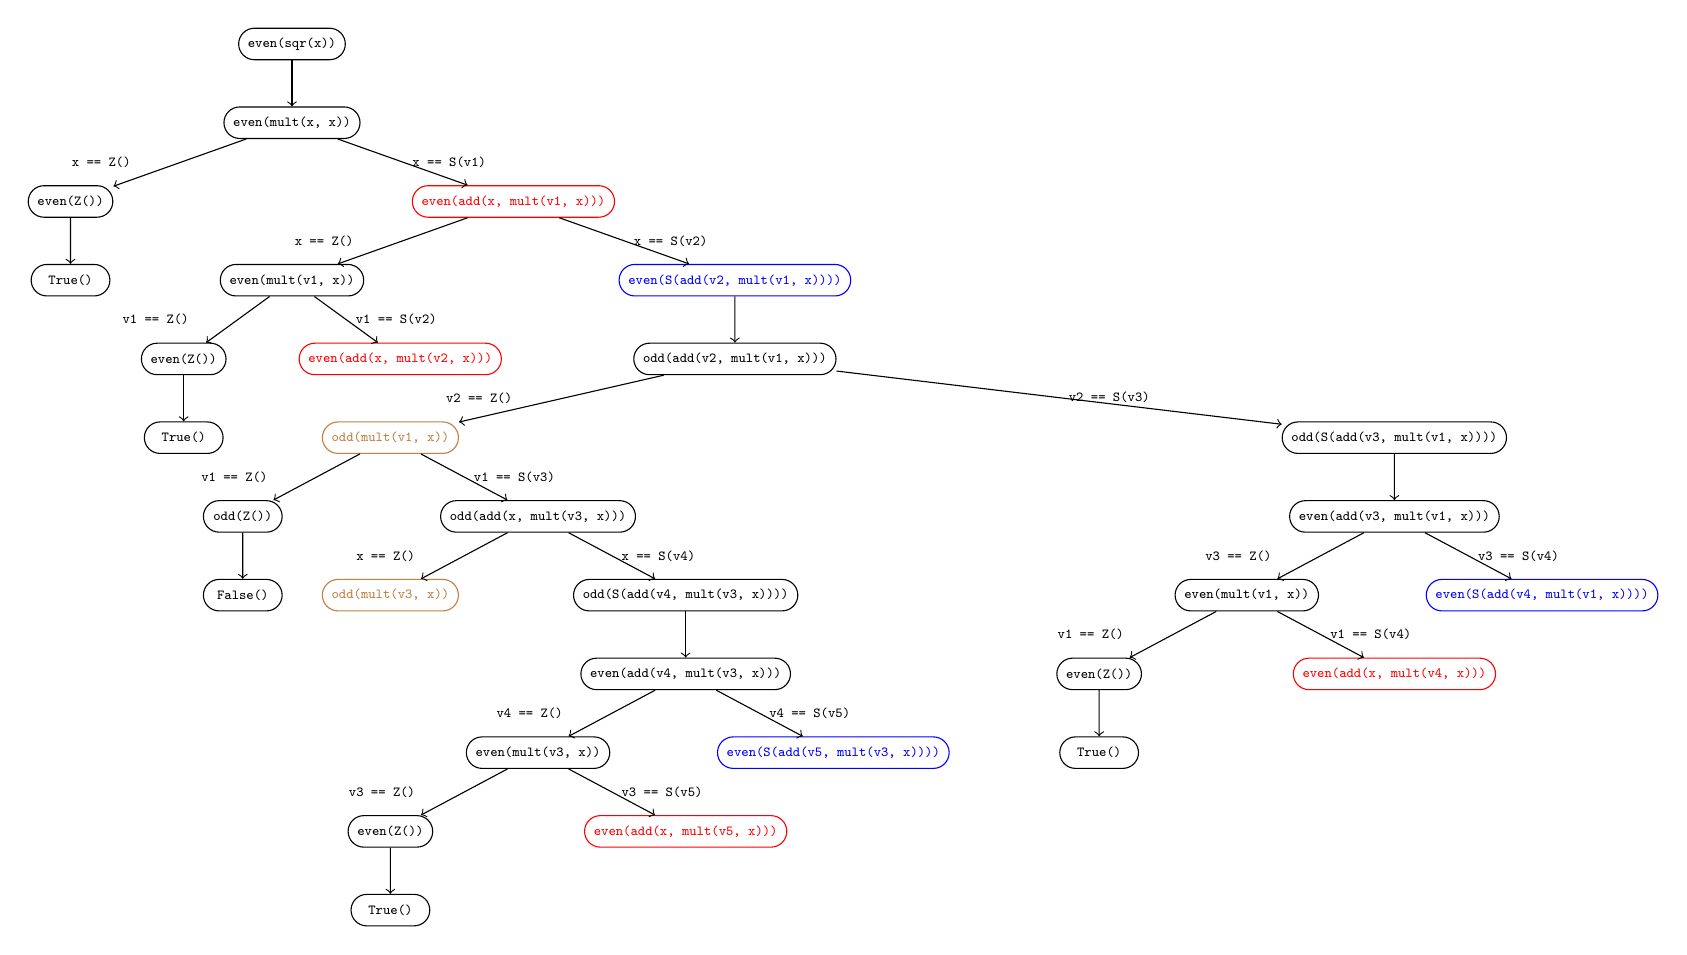
\begin{tikzpicture}[scale=1.25,
level distance=8mm,
level/.style={sibling distance=20mm},
conf/.style={
	rectangle,minimum width=10mm,minimum height=4mm,rounded corners=2mm,
	draw=black,
	font=\ttfamily\tiny},
label/.style={font=\ttfamily\tiny}
]
\tikzstyle{level 2}=[sibling distance=45mm]
\tikzstyle{level 3}=[sibling distance=45mm]
\tikzstyle{level 4}=[sibling distance=22mm]
\tikzstyle{level 5}=[sibling distance=70mm]
\tikzstyle{level 6}=[sibling distance=30mm]
\tikzstyle{level 7}=[sibling distance=30mm]
\tikzstyle{level 8}=[sibling distance=30mm]
\tikzstyle{level 9}=[sibling distance=30mm]
\tikzstyle{level 10}=[sibling distance=30mm]
\node[conf]{even(sqr(x))}
child[->]{node[conf]{even(mult(x, x))}
child[->]{node[conf]{even(Z())}
child[->]{node[conf]{True()}}
edge from parent node[left,label,xshift=-5mm]{x == Z()}}
child[->]{node[conf,red]{even(add(x, mult(v1, x)))}
child[->]{node[conf]{even(mult(v1, x))}
child[->]{node[conf]{even(Z())}
child[->]{node[conf]{True()}}
edge from parent node[left,label,xshift=-5mm]{v1 == Z()}}
child[->]{node[conf,red]{even(add(x, mult(v2, x)))}
edge from parent node[right,label]{v1 == S(v2)}}
edge from parent node[left,label,xshift=-5mm]{x == Z()}}
child[->]{node[conf,blue]{even(S(add(v2, mult(v1, x))))}
child[->]{node[conf]{odd(add(v2, mult(v1, x)))}
child[->]{node[conf,brown]{odd(mult(v1, x))}
child[->]{node[conf]{odd(Z())}
child[->]{node[conf]{False()}}
edge from parent node[left,label,xshift=-5mm]{v1 == Z()}}
child[->]{node[conf]{odd(add(x, mult(v3, x)))}
child[->]{node[conf,brown]{odd(mult(v3, x))}
edge from parent node[left,label,xshift=-5mm]{x == Z()}}
child[->]{node[conf]{odd(S(add(v4, mult(v3, x))))}
child[->]{node[conf]{even(add(v4, mult(v3, x)))}
child[->]{node[conf]{even(mult(v3, x))}
child[->]{node[conf]{even(Z())}
child[->]{node[conf]{True()}}
edge from parent node[left,label,xshift=-5mm]{v3 == Z()}}
child[->]{node[conf,red]{even(add(x, mult(v5, x)))}
edge from parent node[right,label]{v3 == S(v5)}}
edge from parent node[left,label,xshift=-5mm]{v4 == Z()}}
child[->]{node[conf,blue]{even(S(add(v5, mult(v3, x))))}
edge from parent node[right,label]{v4 == S(v5)}}}
edge from parent node[right,label]{x == S(v4)}}
edge from parent node[right,label]{v1 == S(v3)}}
edge from parent node[left,label,xshift=-5mm]{v2 == Z()}}
child[->]{node[conf,xshift=40mm]{odd(S(add(v3, mult(v1, x))))}
child[->]{node[conf]{even(add(v3, mult(v1, x)))}
child[->]{node[conf]{even(mult(v1, x))}
child[->]{node[conf]{even(Z())}
child[->]{node[conf]{True()}}
edge from parent node[left,label,xshift=-5mm]{v1 == Z()}}
child[->]{node[conf,red]{even(add(x, mult(v4, x)))}
edge from parent node[right,label]{v1 == S(v4)}}
edge from parent node[left,label,xshift=-5mm]{v3 == Z()}}
child[->]{node[conf,blue]{even(S(add(v4, mult(v1, x))))}
edge from parent node[right,label]{v3 == S(v4)}}}
edge from parent node[right,label]{v2 == S(v3)}}}
edge from parent node[right,label]{x == S(v2)}}
edge from parent node[right,label]{x == S(v1)}}}
;

\end{tikzpicture}
\end{landscape}

\section{\texttt{Generator.hs}}

The module \texttt{Generator} is quite big, and full of technical details,
mostly related to working with names
\begin{lstlisting}[name=generator]
residuate :: Graph Conf -> Task
residuate tree = (expr, program) where
	(expr, program, _) = res nameSupply [] tree

res :: NameSupply -> [(Conf, Conf)] -> Graph Conf 
	-> (Conf, Program, NameSupply)
res ns mp (Node e Stop) = (e, Program [] [], ns)

res ns mp (Node (Ctr cname _) (Decompose ts)) = 
	(Ctr cname args, p1, ns1) where
		(args, p1, ns1) = res' ns mp ts

res ns mp (Node (Let (v, _) _) (Decompose ts)) = 
	(e2 // [(v, e1)], p1, ns1) where
		([e1, e2], p1, ns1) = res' ns mp ts

res (n:ns) mp (Node e (Transient t)) = 
	(fcall, Program ((FDef f1 vs body):fs) gs, ns1) where
		vs = vnames e
		f1 = "f" ++ (tail n)
		fcall = FCall f1 $ map Var vs
		(body, Program fs gs, ns1) = 
			res ns ((e, fcall) : mp) t

res (n:ns) mp (Node e (Variants cs)) = 
	(gcall, Program fs (newGs ++ gs), ns1) where
		vs@(pv:vs') = vnames e
		(vs_, vs'_) = 
			if (isRepeated pv e) && (isUsed pv cs) 
			then (pv:vs, vs) else (vs, vs')
		g1 = "g" ++ (tail n)
		gcall = GCall g1 $ map Var vs_
		(bodies, Program fs gs, ns1) = 
			res' ns ((e, gcall) : mp) $ map snd cs
		pats = [pat | (Contract v pat, _) <- cs]
		newGs = [GDef g1 p vs'_ b | 
				 (p, b) <-  (zip pats bodies)]
		isUsed vname cs = 
			any (any (== vname) . vnames . nodeLabel . snd) 
				cs

res ns mp (Node e (Fold (Node base _) ren)) = 
	(call, Program [] [], ns) where
		call = baseCall // [(x, Var y) | (x, y) <- ren]
		Just baseCall = lookup base mp

res' :: NameSupply -> [(Conf, Conf)] -> [Graph Conf] 
	-> ([Conf], Program, NameSupply)
res' ns mp ts = foldl f ([], Program [] [], ns) ts where
	f (cs, Program fs gs, ns1) t = 
		(cs ++ [g], Program (fs ++ fs1) (gs ++ gs1), ns2) 
		where
			(g, Program fs1 gs1, ns2) = res ns1 mp t

isBase e1 (Node _ (Decompose ts)) = 
	or $ map (isBase e1) ts
isBase e1 (Node _ (Variants cs)) = 
	or $ map (isBase e1 . snd) cs
isBase e1 (Node _ (Transient t)) = isBase e1 t
isBase e1 (Node _ (Fold (Node e2 _) _)) = e1 == e2
isBase e1 (Node e2 Stop) = False
\end{lstlisting}

\texttt{residuate} delegates the main part of the work to \texttt{res}, which processes 
the tree top-down, left-to-right.
The result of traversing each subtree is a new configuration and a program
(a list of indifferent and curious function definitions).
The main complication is to ensure a unique name for each
generated function.
A more detailed explanation would probably get too long.
The reader is rather invited to study directly the sources.
To aid understanding, we list the graph obtained for the KMP-test
from the main article, and then repeated the same graph
overlaid with the new generated configurations.

%\newpage
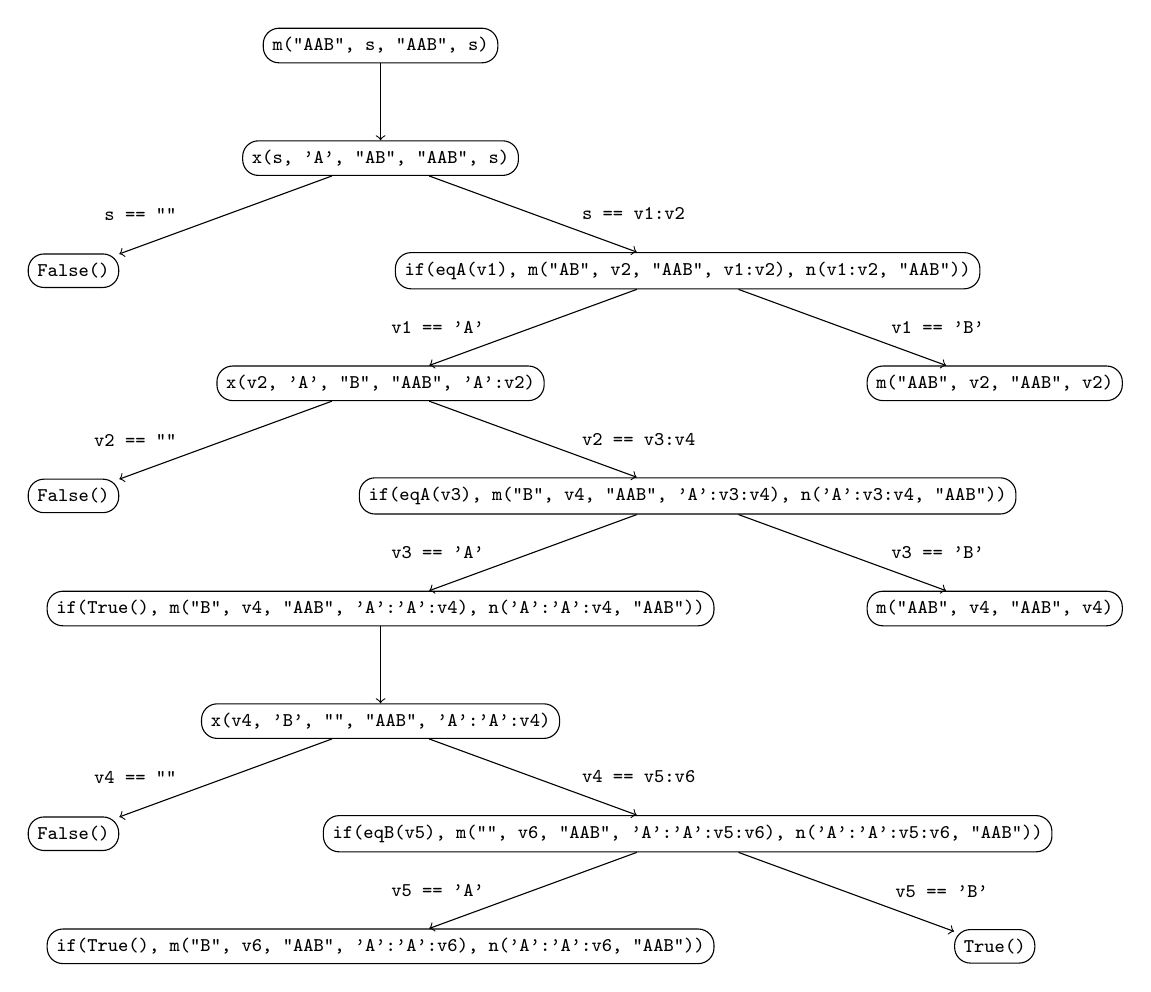
\begin{tikzpicture}[scale=1.3,
level distance=11mm,
level/.style={sibling distance=60mm},
conf/.style={
	rectangle,minimum width=10mm,minimum height=4mm,rounded corners=2mm,
	draw=black,
	font=\ttfamily\scriptsize},
label/.style={font=\ttfamily\scriptsize}
]
% \tikzstyle{level 2}=[sibling distance=45mm]
% \tikzstyle{level 3}=[sibling distance=45mm]
% \tikzstyle{level 4}=[sibling distance=22mm]
% \tikzstyle{level 5}=[sibling distance=70mm]
% \tikzstyle{level 6}=[sibling distance=30mm]
% \tikzstyle{level 7}=[sibling distance=30mm]
% \tikzstyle{level 8}=[sibling distance=30mm]
% \tikzstyle{level 9}=[sibling distance=30mm]
% \tikzstyle{level 10}=[sibling distance=30mm]
\node[conf]{m("AAB", s, "AAB", s)}
child[->]{node[conf]{x(s, 'A', "AB", "AAB", s)}
child[->]{node[conf]{False()}
edge from parent node[left,label,xshift=-5mm]{s == ""}}
child[->]{node[conf]{if(eqA(v1), m("AB", v2, "AAB", v1:v2), n(v1:v2, "AAB"))}
child[->]{node[conf]{x(v2, 'A', "B", "AAB", 'A':v2)}
child[->]{node[conf]{False()}
edge from parent node[left,label,xshift=-5mm]{v2 == ""}}
child[->]{node[conf]{if(eqA(v3), m("B", v4, "AAB", 'A':v3:v4), n('A':v3:v4, "AAB"))}
child[->]{node[conf]{if(True(), m("B", v4, "AAB", 'A':'A':v4), n('A':'A':v4, "AAB"))}
child[->]{node[conf]{x(v4, 'B', "", "AAB", 'A':'A':v4)}
child[->]{node[conf]{False()}
edge from parent node[left,label,xshift=-5mm]{v4 == ""}}
child[->]{node[conf]{if(eqB(v5), m("", v6, "AAB", 'A':'A':v5:v6), n('A':'A':v5:v6, "AAB"))}
child[->]{node[conf]{if(True(), m("B", v6, "AAB", 'A':'A':v6), n('A':'A':v6, "AAB"))}
edge from parent node[left,label,xshift=-5mm]{v5 == 'A'}}
child[->]{node[conf]{True()}
edge from parent node[right,label,xshift=5mm]{v5 == 'B'}}
edge from parent node[right,label,xshift=5mm]{v4 == v5:v6}}}
edge from parent node[left,label,xshift=-5mm]{v3 == 'A'}}
child[->]{node[conf]{m("AAB", v4, "AAB", v4)}
edge from parent node[right,label,xshift=5mm]{v3 == 'B'}}
edge from parent node[right,label,xshift=5mm]{v2 == v3:v4}}
edge from parent node[left,label,xshift=-5mm]{v1 == 'A'}}
child[->]{node[conf]{m("AAB", v2, "AAB", v2)}
edge from parent node[right,label,xshift=5mm]{v1 == 'B'}}
edge from parent node[right,label,xshift=5mm]{s == v1:v2}}}


;

\end{tikzpicture}

%Просто граф.

%\newpage
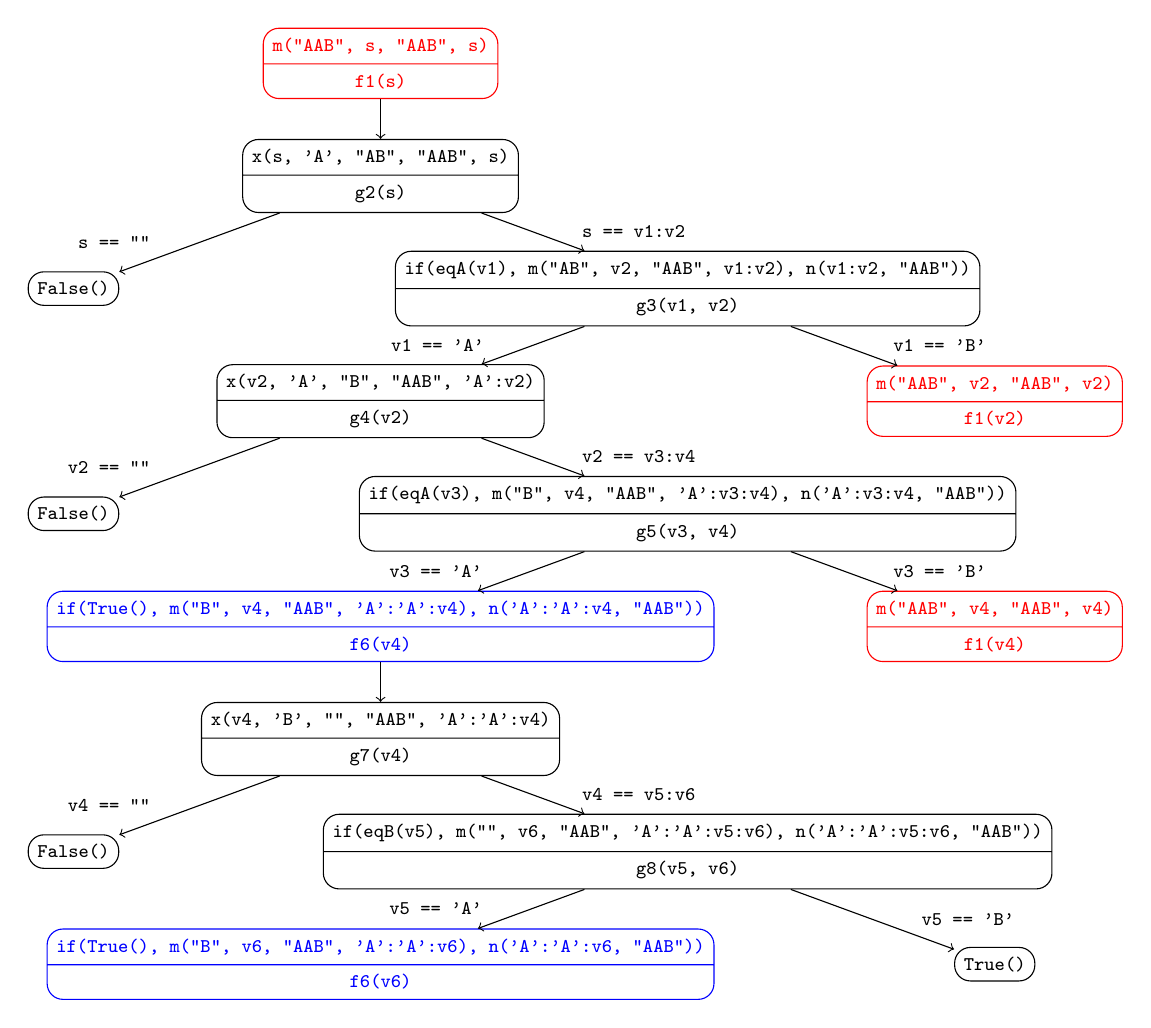
\begin{tikzpicture}[scale=1.3,
level distance=11mm,
level/.style={sibling distance=60mm},
conf/.style={
	rectangle,minimum width=10mm,minimum height=4mm,rounded corners=2mm,
	draw=black,
	font=\ttfamily\scriptsize},
label/.style={font=\ttfamily\scriptsize},
base/.style={
	rectangle split, rectangle split parts=2, draw,rounded corners=2mm,
	draw=black,
	font=\ttfamily\scriptsize},
]
% \tikzstyle{level 2}=[sibling distance=45mm]
% \tikzstyle{level 3}=[sibling distance=45mm]
% \tikzstyle{level 4}=[sibling distance=22mm]
% \tikzstyle{level 5}=[sibling distance=70mm]
% \tikzstyle{level 6}=[sibling distance=30mm]
% \tikzstyle{level 7}=[sibling distance=30mm]
% \tikzstyle{level 8}=[sibling distance=30mm]
% \tikzstyle{level 9}=[sibling distance=30mm]
% \tikzstyle{level 10}=[sibling distance=30mm]
\node[base,red]{m("AAB", s, "AAB", s)\nodepart{second}f1(s)}
child[->]{node[base]{x(s, 'A', "AB", "AAB", s)\nodepart{second}g2(s)}
child[->]{node[conf]{False()}
edge from parent node[left,label,xshift=-5mm]{s == ""}}
child[->]{node[base]{if(eqA(v1), m("AB", v2, "AAB", v1:v2), n(v1:v2, "AAB"))
\nodepart{second}g3(v1, v2)}
child[->]{node[base]{x(v2, 'A', "B", "AAB", 'A':v2)
\nodepart{second}g4(v2)}
child[->]{node[conf]{False()}
edge from parent node[left,label,xshift=-5mm]{v2 == ""}}
child[->]{node[base]{if(eqA(v3), m("B", v4, "AAB", 'A':v3:v4), n('A':v3:v4, "AAB"))
\nodepart{second}g5(v3, v4)}
child[->]{node[base,blue]{if(True(), m("B", v4, "AAB", 'A':'A':v4), n('A':'A':v4, "AAB"))
\nodepart{second}f6(v4)}
child[->]{node[base]{x(v4, 'B', "", "AAB", 'A':'A':v4)
\nodepart{second}g7(v4)}
child[->]{node[conf]{False()}
edge from parent node[left,label,xshift=-5mm]{v4 == ""}}
child[->]{node[base]{if(eqB(v5), m("", v6, "AAB", 'A':'A':v5:v6), n('A':'A':v5:v6, "AAB"))
\nodepart{second}g8(v5, v6)}
child[->]{node[base,blue]{if(True(), m("B", v6, "AAB", 'A':'A':v6), n('A':'A':v6, "AAB"))
\nodepart{second}f6(v6)}
edge from parent node[left,label,xshift=-5mm]{v5 == 'A'}}
child[->]{node[conf]{True()}
edge from parent node[right,label,xshift=5mm]{v5 == 'B'}}
edge from parent node[right,label,xshift=5mm]{v4 == v5:v6}}}
edge from parent node[left,label,xshift=-5mm]{v3 == 'A'}}
child[->]{node[base,red]{m("AAB", v4, "AAB", v4)
\nodepart{second}f1(v4)}
edge from parent node[right,label,xshift=5mm]{v3 == 'B'}}
edge from parent node[right,label,xshift=5mm]{v2 == v3:v4}}
edge from parent node[left,label,xshift=-5mm]{v1 == 'A'}}
child[->]{node[base,red]{m("AAB", v2, "AAB", v2)
\nodepart{second}f1(v2)}
edge from parent node[right,label,xshift=5mm]{v1 == 'B'}}
edge from parent node[right,label,xshift=5mm]{s == v1:v2}}};
\end{tikzpicture}

In the last figure we again mark by the same color nodes, which are equal
up to renaming.
The upper part of each node contains the original configuration,
the lower part -- the new configuration generated by \texttt{res}.

\begin{lstlisting}[style=demo,escapechar=!]
ghci> let g = ...

-- demo24
ghci> residuate g
f1(s)
f1(s) = g2(s);
g2("") = False();
g2(v1:v2) = g3(v1, v2);
g3('A', v2) = g4(v2);
g3('B', v2) = f1(v2);
g4("") = False();
g4(v3:v4) = g5(v3, v4);
g5('A', v4) = f6(v4);
g5('B', v4) = f1(v4);
f6(v4) = g7(v4);
g7("") = False();
g7(v5:v6) = g8(v5, v6);
g8('A', v6) = f6(v6);
g8('B', v6) = True();
\end{lstlisting}
\section{\texttt{Propotype.hs}}

This is the simplest ``prototype'' supercompiler.
No simplification (transient step removal) of the graph is performed, nor information propagation.
\begin{lstlisting}[name=prototype]
transform :: Task -> Task
transform (e, p) =
	residuate $ foldTree $ buildFTree (driveMachine p) e
\end{lstlisting}

\texttt{buildFTree} builds the foldable tree. 
The only difference with \texttt{buildTree} lies in the fact,
that generalization is performed if the whistle blows:
\begin{lstlisting}[name=prototype]
buildFTree :: Machine Conf -> Conf -> Tree Conf
buildFTree m e = bft m nameSupply e

bft :: Machine Conf -> NameSupply -> Conf -> Tree Conf
bft d (n:ns) e | whistle e = bft d ns $ generalize n e
bft d ns     t | otherwise = case d ns t of
	Decompose ds -> Node t $ Decompose $ map (bft d ns) ds
	Transient e -> Node t $ Transient $ bft d ns e
	Stop -> Node t Stop
	Variants cs -> Node t $ 
		Variants [(c, bft d (unused c ns) e) | (c, e) <- cs]
\end{lstlisting}

Probably the simplest possible whistle:
\begin{lstlisting}[name=prototype]
sizeBound = 40
whistle :: Expr -> Bool
whistle e@(FCall _ args) = 
	not (all isVar args) && size e > sizeBound
whistle e@(GCall _ args) = 
	not (all isVar args) && size e > sizeBound
whistle _ = False
\end{lstlisting}

Generalization is also extremely simple, compared to most other supercompilers --
the biggest subexpression is lifted into a \texttt{let} for separate processing:
\begin{lstlisting}[name=prototype]
generalize :: Name -> Expr -> Expr
generalize n (FCall f es) =
	Let (n, e) (FCall f es') where 
		(e, es') = extractArg n es
generalize n (GCall g es) =
	Let (n, e) (GCall g es') where 
		(e, es') = extractArg n es

extractArg :: Name -> [Expr] -> (Expr, [Expr])
extractArg n es = (maxE, vs ++ Var n : ws) where
	maxE = maximumBy ecompare es
	ecompare x y = 
		compare (eType x * size x) (eType y * size y)
	(vs, w : ws) = break (maxE ==) es
	eType e = if isVar e then 0 else 1
\end{lstlisting}

\section{\texttt{Deforester.hs}}
If we just add \texttt{simplify} (transient edge removal) to the text of \texttt{transform},
we obtain deforestation:
\begin{lstlisting}[name=deforester]
deforest :: Task -> Task
deforest (e, p) =
	residuate $ simplify $ foldTree $ 
		buildFTree (driveMachine p) e

simplify :: Graph Conf -> Graph Conf
simplify (Node e (Decompose ts)) =
	Node e (Decompose $ map simplify ts)
simplify (Node e (Variants cs)) =
	Node e (Variants [(c, simplify t) | (c, t) <- cs])
simplify (Node e (Transient t)) | isBase e t =
	Node e $ Transient $ simplify t
simplify (Node e (Transient t)) =
	simplify t
simplify t = t
\end{lstlisting}
\section{\texttt{Supercompiler.hs}}

As a next step, we extend deforestation with information propagation,
to obtain our final supercompiler:
\begin{lstlisting}[name=supercompiler]
supercompile :: Task -> Task
supercompile (e, p) =
	residuate $ simplify $ foldTree $ 
		buildFTree (addPropagation $ driveMachine p) e

addPropagation :: Machine Conf -> Machine Conf
addPropagation m ns e = propagateContract (m ns e)

propagateContract :: Step Conf -> Step Conf
propagateContract (Variants vs) =
  Variants [(c, e // [(v, Ctr cn $ map Var vs)]) | 
            (c@(Contract v (Pat cn vs)), e) <- vs]
propagateContract step = step
\end{lstlisting}

The reader is encouraged to compare the trees produced by different transformers:

\begin{lstlisting}[style=demo,escapechar=!]
-- demo21
ghci> foldTree $ buildFTree (driveMachine prog2) 
	{{match("AAB", s)}}
...

-- demo22
ghci> simplify $ foldTree $ buildFTree (driveMachine prog2) 
	{{match("AAB", s)}}
...

-- demo23
ghci> simplify $ foldTree $ buildFTree (addPropagation 
(driveMachine prog2)) conf2
...
\end{lstlisting}

\ldots and also the resulting residual tasks (listed also in the main article):
\begin{lstlisting}[style=demo,escapechar=!]
-- demo24
ghci> transform ({{match("AAB", s)}}, prog2)
...

-- demo25
ghci> deforest ({{match("AAB", s)}}, prog2)
...

-- demo26
ghci> supercompile ({{match("AAB", s)}}, prog2)
...
\end{lstlisting}

\section{Anti-KMP test}

This section lists in detail the results of the anti-KMP-test mentioned in the main text.
To improve readability, we set specifically for these examples \texttt{sizeBound=10}.

The baseline transformer produces 19 functions.
\begin{lstlisting}[style=demo,escapechar=!]
-- demo18
ghci> transform ({{even(sqr(x))}}, prog1)
f1(x)
f1(x) = g2(x, x);
f3() = True();
f6() = True();
f7(v2, v1, x) = g8(v2, v1, x);
f10() = False();
f12(v4, v3, x) = g13(v4, v3, x);
f15() = True();
f16(v3, v1, x) = g17(v3, v1, x);
f19() = True();
g2(Z(), x) = f3();
g2(S(v1), x) = g4(x, x, v1);
g4(Z(), x, v1) = g5(v1, x);
g4(S(v2), x, v1) = f7(v2, v1, x);
g5(Z(), x) = f6();
g5(S(v2), x) = g4(x, x, v2);
g8(Z(), v1, x) = g9(v1, x);
g8(S(v3), v1, x) = f16(v3, v1, x);
g9(Z(), x) = f10();
g9(S(v3), x) = g11(x, x, v3);
g11(Z(), x, v3) = g9(v3, x);
g11(S(v4), x, v3) = f12(v4, v3, x);
g13(Z(), v3, x) = g14(v3, x);
g13(S(v5), v3, x) = f7(v5, v3, x);
g14(Z(), x) = f15();
g14(S(v5), x) = g4(x, x, v5);
g17(Z(), v1, x) = g18(v1, x);
g17(S(v4), v1, x) = f7(v4, v1, x);
g18(Z(), x) = f19();
g18(S(v4), x) = g4(x, x, v4);
\end{lstlisting}

Deforestation -- 11 functions:
\begin{lstlisting}[style=demo,escapechar=!]
-- demo19
ghci> deforest ({{even(sqr(x))}}, prog1)
g1(x, x)
f4(v2, v1, x) = g5(v2, v1, x);
g1(Z(), x) = True();
g1(S(v1), x) = g2(x, x, v1);
g2(Z(), x, v1) = g3(v1, x);
g2(S(v2), x, v1) = f4(v2, v1, x);
g3(Z(), x) = True();
g3(S(v2), x) = g2(x, x, v2);
g5(Z(), v1, x) = g6(v1, x);
g5(S(v3), v1, x) = g10(v3, v1, x);
g6(Z(), x) = False();
g6(S(v3), x) = g7(x, x, v3);
g7(Z(), x, v3) = g6(v3, x);
g7(S(v4), x, v3) = g8(v4, v3, x);
g8(Z(), v3, x) = g9(v3, x);
g8(S(v5), v3, x) = f4(v5, v3, x);
g9(Z(), x) = True();
g9(S(v5), x) = g2(x, x, v5);
g10(Z(), v1, x) = g11(v1, x);
g10(S(v4), v1, x) = f4(v4, v1, x);
g11(Z(), x) = True();
g11(S(v4), x) = g2(x, x, v4);
\end{lstlisting}

%\newpage
Supercompilation -- 34 functions.
\begin{lstlisting}[style=demo,escapechar=!]
-- demo20
ghci> supercompile ({{even(sqr(x))}}, prog1)
g1(x)
g1(Z()) = True();
g1(S(v1)) = g2(v1);
g2(Z()) = False();
g2(S(v2)) = g3(v2);
g3(Z()) = True();
g3(S(v3)) = g33(S(g4(v3)));
g4(Z()) = S(S(S(S(S(S(Z()))))));
g4(S(v5)) = S(g32(v5, S(S(S(S(g31(v5, S(S(S(S(g30(v5, 
	S(S(S(S(g29(v5, g5(v5))))))))))))))))));
g5(Z()) = Z();
g5(S(v10)) = S(S(S(S(S(g28(v10, g6(v10)))))));
g6(Z()) = Z();
g6(S(v12)) = S(S(S(S(S(S(g27(v12, g7(v12))))))));
g7(Z()) = Z();
g7(S(v14)) = S(S(S(S(S(S(S(g26(v14, g8(v14)))))))));
g8(Z()) = Z();
g8(S(v16)) = g25(S(S(S(S(S(S(S(S(v16)))))))), 
	g9(v16, S(S(S(S(S(S(S(S(v16))))))))));
g9(Z(), v18) = Z();
g9(S(v19), v18) = g10(v18, v19);
g10(Z(), v19) = g11(v19);
g10(S(v20), v19) = S(g12(v20, v19));
g11(Z()) = Z();
g11(S(v20)) = g11(v20);
g12(Z(), v19) = g13(v19);
g12(S(v21), v19) = S(g14(v21, v19));
g13(Z()) = Z();
g13(S(v21)) = S(g13(v21));
g14(Z(), v19) = g15(v19);
g14(S(v22), v19) = S(g16(v22, v19));
g15(Z()) = Z();
g15(S(v22)) = S(S(g15(v22)));
g16(Z(), v19) = g17(v19);
g16(S(v23), v19) = S(g18(v23, v19));
g17(Z()) = Z();
g17(S(v23)) = S(S(S(g17(v23))));
g18(Z(), v19) = g19(v19);
g18(S(v24), v19) = S(g20(v24, v19));
g19(Z()) = Z();
g19(S(v24)) = S(S(S(S(g19(v24)))));
g20(Z(), v19) = g21(v19);
g20(S(v25), v19) = S(g24(v25, g22(v19, v25)));
g21(Z()) = Z();
g21(S(v25)) = S(S(S(S(S(g21(v25))))));
g22(Z(), v25) = Z();
g22(S(v27), v25) = S(S(S(S(S(S(g23(v25, g22(v27, 
	v25))))))));
g23(Z(), v28) = v28;
g23(S(v29), v28) = S(g23(v29, v28));
g24(Z(), v26) = v26;
g24(S(v27), v26) = S(g24(v27, v26));
g25(Z(), v17) = v17;
g25(S(v19), v17) = S(g25(v19, v17));
g26(Z(), v15) = v15;
g26(S(v16), v15) = S(g26(v16, v15));
g27(Z(), v13) = v13;
g27(S(v14), v13) = S(g27(v14, v13));
g28(Z(), v11) = v11;
g28(S(v12), v11) = S(g28(v12, v11));
g29(Z(), v9) = v9;
g29(S(v10), v9) = S(g29(v10, v9));
g30(Z(), v8) = v8;
g30(S(v9), v8) = S(g30(v9, v8));
g31(Z(), v7) = v7;
g31(S(v8), v7) = S(g31(v8, v7));
g32(Z(), v6) = v6;
g32(S(v7), v6) = S(g32(v7, v6));
g33(Z()) = True();
g33(S(v5)) = g34(v5);
g34(Z()) = False();
g34(S(v6)) = g33(v6);
\end{lstlisting}

We compare below the speed-ups of the task \texttt{{\color{brown}even(sqr(x))}, prog1}
obtained by using \texttt{transform}, \texttt{deforest}, and \texttt{supercompile}.
The speed-up of task $t_2$ with respect to task $t_1$ is calculated
as follows (where \texttt{x} is a natural number, and \texttt{{\color{brown}x}} -- the corresponding Peano number):

\begin{lstlisting}[style=demo]
acc t1 t2 x = steps1 / steps2 where
	(_, steps1) = sll_trace t1 [("x"), {{x}}]
	(_, steps2) = sll_trace t2 [("x"), {{x}}]
\end{lstlisting}

\newpage
\begin{tikzpicture}[yscale=2,xscale=0.25]
%\draw[very thin,color=gray] (-0.1,-0.1) grid (40,5.1);
\draw[->] (-0.2,0) -- (41,0) node[right] {$x$};
\draw[->] (0,-0.05) -- (0,5.2) node[above] {$acc(x)$};
% just transformation
\draw[] plot[mark=*, mark options={yscale=0.4,xscale=2,color=red}] coordinates
{(0,1.0) (1,1.0) (2,1.0) (3,1.0) (4,1.0) (5,1.0)
(6,1.0) (7,1.0) (8,1.0) (9,1.0) (10,1.0) (11,1.0) (12,1.0) (13,1.0) (14,1.0) (15,1.0) (16,1.0) (17,1.0) (18,1.0) (19,1.0)
(20,1.0) (21,1.0) (22,1.0) (23,1.0) (24,1.0) (25,1.0) (26,1.0) (27,1.0) (28,1.0) (29,1.0) (30,1.0)
(31,1.0) (32,1.0) (33,1.0) (34,1.0) (35,1.0) (36,1.0) (37,1.0) (38,1.0) (39,1.0) (40,1.0)}
node[right,xshift=0.5cm,red]{\texttt{transform}};

% deforestation
\draw[] plot[mark=*, mark options={yscale=0.4,xscale=2, color=blue}] coordinates
{(0,3.0) (1,1.4) (2,1.3636363636363635) (3,1.2857142857142858) (4,1.303030303030303)
(5,1.2857142857142858) (6,1.2985074626865671) (7,1.2921348314606742) (8,1.3008849557522124)
(9,1.297872340425532) (10,1.304093567251462) (11,1.302439024390244) (12,1.3070539419087137)
(13,1.3060498220640568) (14,1.3095975232198143) (15,1.3089430894308942) (16,1.3117505995203838)
(17,1.3113006396588487) (18,1.3135755258126196) (19,1.3132530120481927) (20,1.3151326053042123)
(21,1.3148936170212766) (22,1.3164721141374838) (23,1.3162901307966706) (24,1.3176341730558598)
(25,1.3174924165824065) (26,1.3186504217432053) (27,1.318537859007833) (28,1.3195458231954582)
(29,1.3194549583648751) (30,1.3203401842664777) (31,1.320265780730897) (32,1.3210493441599)
(33,1.3209876543209877) (34,1.3216860787576261) (35,1.321634363541121) (36,1.3222607833415965)
(37,1.3222170032879286) (38,1.3227819884083816) (39,1.3227445997458704) (40,1.3232567513099556)}
node[right,xshift=0.5cm,yshift=0.5cm,blue]{\texttt{deforest}};

% supercompilation
\draw[] plot[mark=*, mark options={yscale=0.4,xscale=2, color=orange}] coordinates
{(0,3.0) (1,3.5) (2,5.0) (3,2.25) (4,1.7916666666666667) (5,1.6153846153846154)
(6,1.5263157894736843) (7,1.4743589743589745) (8,1.3363636363636364) (9,1.2534246575342465)
(10,1.238888888888889) (11,1.224770642201835) (12,1.2115384615384615) (13,1.1993464052287581)
(14,1.1882022471910112) (15,1.1780487804878048) (16,1.1688034188034189) (17,1.1603773584905661)
(18,1.1526845637583893) (19,1.1456456456456456) (20,1.1391891891891892) (21,1.1332518337408313)
(22,1.1277777777777778) (23,1.1227180527383367) (24,1.1180297397769516) (25,1.1136752136752137)
(26,1.109621451104101) (27,1.1058394160583942) (28,1.1023035230352303) (29,1.0989911727616646)
(30,1.0958823529411765) (31,1.092959295929593) (32,1.0902061855670102) (33,1.0876089060987415)
(34,1.0851548269581057) (35,1.082832618025751) (36,1.0806320907617504) (37,1.078544061302682)
(38,1.0765602322206096) (39,1.0746730901582933) (40,1.072875816993464)}
node[right,xshift=0.5cm,yshift=0.4cm,orange]{\texttt{supercompile}};

\foreach \x in {0,5,10,...,40} \draw (\x cm,1pt) -- (\x cm,-1pt) node[anchor=north] {$\x$};
\foreach \x in {0.5,1,...,5} \draw (1pt,\x cm) -- (-1pt,\x cm) node[anchor=east] {$\x$};
\end{tikzpicture}


These results demonstrate, that the speed-up from supercompilation is most impressive
for small $x$;
for such small numbers we do not reach the cases of generalization present in the graph.
When $х$ grows, however, the drawbacks of performing generalization start to show,
and the deforested task turns out faster.

%\begin{exercise}
%То, что суперкомпиляция может выдавать программы, работающие медленнее, чем дефорестированные,
%даже при ``идеальной'' модели стоимости вычисления (у нас скорость вычислений измерялась в шагах
%интерпретатора), было для меня поначалу большим сюрпризом. Задание объяснить, как такое возможно,
%достается в качестве награды самому любопытному и дотошному читателю, добравшемуся до конца этого
%опуса.
%\end{exercise}


\end{document}